%%%%%%%%%%%%%%%%%%%%%%%%%%%%%%%%%%%%%%%%%
% University Assignment Title Page 
% LaTeX Template
% Version 1.0 (27/12/12)
%
% This template has been downloaded from:
% http://www.LaTeXTemplates.com
%
% Original author:
% WikiBooks (http://en.wikibooks.org/wiki/LaTeX/Title_Creation)
%
% License:
% CC BY-NC-SA 3.0 (http://creativecommons.org/licenses/by-nc-sa/3.0/)
%
%%%%%%%%%%%%%%%%%%%%%%%%%%%%%%%%%%%%%%%%%
%\title{Title page with logo}
%----------------------------------------------------------------------------------------
%	PACKAGES AND OTHER DOCUMENT CONFIGURATIONS
%----------------------------------------------------------------------------------------

\documentclass[12pt]{article}
\usepackage[english]{babel}
\usepackage[utf8]{inputenc}
\usepackage{natbib}
\usepackage{amsmath}
\usepackage{color}
\usepackage[explicit]{titlesec}
\usepackage[hyphens,spaces,obeyspaces]{url}
\usepackage{graphicx}
\usepackage{grffile}
\usepackage{placeins}

\usepackage{pgfplots}
\usepackage{tikz,tikz-3dplot}
\usepgfplotslibrary{colormaps,fillbetween}
\pgfplotsset{compat=1.16}
%	\pgfplotscolormaptoshadingspec{hot}{7cm}\result
%	\def\tempb{\pgfdeclarehorizontalshading{tempshading}{7cm}}%
%	% where '\result' is inserted as last argument:
%	\expandafter\tempb\expandafter{\result}%
%	\sbox\backbox{\pgfuseshading{tempshading}}%

\counterwithin*{section}{part}


\begin{document}

\begin{titlepage}

\newcommand{\HRule}{\rule{\linewidth}{0.5mm}} % Defines a new command for the horizontal lines, change thickness here

\center % Center everything on the page
 
%----------------------------------------------------------------------------------------
%	HEADING SECTIONS
%----------------------------------------------------------------------------------------

\textsc{\LARGE University of St Andrews}\\[1.5cm] % Name of your university/college
\textsc{\Large CS4099}\\[0.5cm] % Major heading such as course name
\textsc{\large }\\[0.5cm] % Minor heading such as course title

%----------------------------------------------------------------------------------------
%	TITLE SECTION
%----------------------------------------------------------------------------------------

\HRule \\[0.4cm]
{ \huge \bfseries ILNP Routing for IoT}\\[0.4cm] % Title of your document
\HRule \\[1.5cm]
 
%----------------------------------------------------------------------------------------
%	AUTHOR SECTION
%----------------------------------------------------------------------------------------


\Large \emph{Author:}\\
 \textsc{Jordan Mackie}\\[1cm] % Your name
 
\Large \emph{Supervisor:}\\
 \textsc{Prof Saleem Bhatti}\\[1cm] % Your name
%----------------------------------------------------------------------------------------
%	DATE SECTION
%----------------------------------------------------------------------------------------

{\large \today}\\[2cm] % Date, change the \today to a set date if you want to be precise

%----------------------------------------------------------------------------------------
%	LOGO SECTION
%---------------------------------------------------------------------------------------


\includegraphics[width = 2.5cm]{images/standrewslogo.png}
 
%----------------------------------------------------------------------------------------

\vfill % Fill the rest of the page with whitespace

\end{titlepage}

\pagenumbering{gobble}

\part*{Abstract}

This project provides an implementation of a wireless ad-hoc sensor network, using ILNP as an addressing scheme. It focuses on an agricultural scenario, where groups of sensors are able to monitor and manage their local environment, whilst also providing data to a sink node for more in depth analysis. A zoning approach was taken to route data through the WSN, where subnetworks were created within the WSN in order to provide energy effecient routing with low memory and communication overhead. Finally, an experiment is carried out to show how effective the protocol is when using ILNP and IP as an addressing scheme, and also evaluates the effectiveness of the protocol along. The results showed that ...

\part*{Declaration}
I declare that the material submitted for
assessment is my own work except where credit is
explicitly given to others by citation or
acknowledgement. This work was performed during
the current academic year except where otherwise
stated.
The main text of this project report is \#TODO NN,NNN
words long, including project specification and plan.
In submitting this project report to the University of
St Andrews, I give permission for it to be made
available for use in accordance with the regulations of
the University Library. I also give permission for
the title and abstract to be published and for copies of
the report to be made and supplied at cost to any bona
fide library or research worker, and to be made
available on the World Wide Web. I retain the
copyright in this work.

\newpage

\tableofcontents

\newpage
\pagenumbering{arabic}
\setcounter{page}{1} 

\section{Introduction}

Despite the imminent exhaustion of IPv4 addresses \cite{ripe_labs}, IPv6 is still being adopted slowly \cite{google_ipv6}. Brittle solutions such as NAT are being used to expand the IPv4 address space and to avoid the transition costs involved in upgrading to IPv6. Whilst IPv6 does expand the address space greatly and introduces functionality such as multicast, the internet protocol has more intrinsic issues. The initial design for the infrastructure of the internet did not account for level of mobility that is common with network capable devices nowadays, and the attempts to retrospectively include support for such features have resulted in an incredibly complex system made of incompatible components. 

IP addresses are used both to identify a system and to determine its topological location. \cite{briancarpenter2014} lists several of the downsides to this overloading of IP addresses, and why the protocol was still adopted despite them.

The separation of concerns that should be achieved by a layered model is not possible, since the IP address is used by each layer in some way. IP addresses can be used in the application layer, and are bound to physical network interfaces, which goes against the end-to-end argument where each layer should provide a opaque abstraction to those above it.

The issues with IP are not just semantic. Due to the overloading of the IP address and the rapid increase in internet connected devices \cite{iot_stat}, the scalability of the system is being challenged. Implementations of multipath routing with the intention of balancing load is improving network performance for the operators that use them, but with IP it places greater stress on the default-free zone (DFZ) routing information base (RIB). Multihoming is also being used to improve reliability, but with IP this requires routing entries to store multiple addresses for one host. An IAB workshop \cite{rfc4984} detailed how the DFZ RIB databases are growing in size exponentially due to the increasing number of devices and an inability to aggregate address prefixes. With IPv6 allowing for an even larger address space, this problem will only get worse. 

As the number of Internet of Things (IoT) devices grows, mobility is also becoming a necessary feature for a networking protocol. Mobile IP currently requires another entity (a home agent) to track and proxy packets to the mobile host as it moves from network to network. This mobility is also problematic for IPSec, which requires that the end system addresses remain fixed.

IoT devices are often restricted by limited battery life, memory, and computational capabilities. Most IP routing protocols focus on finding the shortest route between a source and destination, which often results in a small number of paths being heavily used and so some nodes are especially drained due to processing and forwarding of packets. Mobility of nodes also requires more update messages to be flooded throughout networks. This can result in a network partion once crucial nodes fail (due to loss of battery), rendering a section of still operational nodes useless. A different approach to routing and addressing that reduced the networking overhead and attempted to balance traffic across several paths would allow IoT networks to remain operational for longer. 

Given the difficulty involved in simply migrating from IPv4 to IPv6, it is very doubtful that introducing an entirely different protocol for the internet would be successful. A backwards compatible solution would likely be the only solution that would be adopted within a reasonable time frame.

Both multihoming and mobility are far simpler to implement and maintain if the identity and topological locator of a host are separated, and this is how the Identifier-Locator Network Protocol functions. \cite{5586444} proposes ILNPv6, which implement ILNP with the same address space as IPv6 and the same packet structure as IPv6, but with different semantics for interpreting the addresses. ILNPv6 splits the original 128-bits used for an IPv6 address into two 64-bit fields: the upper bits representing the locator and the lower 64 bits representing the identifier. The version field in the IP header is used to differentiate between ILNPv6 and IPv6 packets, and routers that don't support ILNP can interpret the packets as IP without any issue. 

The locator value identifies the subnetwork that a host belongs to, and a host can have multiple locator values, providing multihoming with smaller memory requirements for the RIB. The ID part of the address is unique to the host, and provides a fixed address which can be used at the transport layer.

Though ILNPv6 is very backwards-compatible, there are still some difficult challenges involved in its deployment. \cite{ipwithoutip} describes how the tight coupling of the C socket API and IP addresses could cause issues in some legacy applications. ILNPv6 also requires some additions to the Domain Name System (DNS) to properly support multihoming.

The main goal of this project is to produce a library for a prototype communication
protocol for Internet of Things (IoT) devices based on the identifier-locator
approach. 

By providing a libary for future developers and researchers to use, the adoptation of ILNP could be accelerated. The native support for multihoming and multipath routing is especially beneficial to typically mobile internet of things (IoT) devices, and so this project aims to exemplify these benefits for agricultural sensor networks in particular. 

\vspace{\baselineskip}
\noindent A sucessful implementation would include:

\begin{enumerate}
	\item \textbf{Load Balancing}: The protocol will attempt to evenly disperse load across a network of IoT
devices. This could be measured by demonstrating a reasonably even distribution of packets throughout the network of nodes when simulating sensor traffic. 
	\item \textbf{Soft Handovers}: The protocol will attempt to handle ’soft-handovers’, allowing nodes to
move between subnetworks and handle node failure without a noticeable effect on performance. A successful implementation will recover from failed nodes, with messages still arriving reliably. This could be tested by emulating network traffic, and triggering nodes in certain positions in the network topology to fail.

\item \textbf{IoT Optimization}: The protocol will account for battery usage on devices to reduce energy drain
on devices. This will be tested through emulation of an IoT network and the energy cost of packets.
\end{enumerate}

\pagebreak
\section{Context Survey}

Despite the intitial motivation for WSNs being military applications, they are now being used to solve many other problems.

The sensitivity of crops to changes in climate and agricultures crucial role on national economies has naturally resulted in large amounts of research and development. \cite{agrisensor} describe how sensor technology is being used to monitor conditions in greenhouses, fields, and bodies of water. In order to make accessing this data more convenient and to help automate processes, they implemented a wireless network of enviromental sensors. This data would then be collected at a sink node and could be analysed from an application. 

WSNs currently often require specialised applications and manually specified network configurations in order for consumers to collect and analyse the data they produce. In order to make access to the data more standardised and easily available, research is also being done to connect sensor networks to the cloud. \cite{indoor} propose enviromental sensors for urban environments with gateways to to the internet which could integrate into our own homes. By providing cheap montoring and actuating sensors to the general public, they hope to encourage healthier eating habits, as people would be able to grow their own vegetables effectively. 

\cite{wsnlist} list the other applications of WSNs, and the different approaches to integrating WSNs and the internet. They recognise that providing a single gateway results in a single point of failure, and so focus on methods involving multiple or integrated gateways. This requires that sensors adopt the responsiblity of managing their networks topology instead of just forwarding towards a sink node. 

Previous research involving integrating WSNs into the current internet infrastructure is typically structured around IP. For all the reasons mentioned earlier, researches have realised the benefits of building WSNs using other approaches such as the locator-identifier split.

In RFC6115 \cite{rfc6115}, ILNP was listed alongside several other solutions that resolved the issues faced by IP. One of the most well researched solutions listed is the Locator-Identifer Split Protocol (LISP), which has already been deployed in 60 sites over 10 countries \cite{nahla}. Whilst it does not have natural support for network mobility, attempts have been made to provide it that require further extensions to the protocol \cite{moblisp}. 

ILNPv6 on the other hand has been able to demonstrate reliable mobility using a soft handover process \cite{shilnp}. Soft handover is where a host remains connected to it's original network while transitioning to a new one, which avoids loss of data when packets are still being routed to it's original network. 

Soft handovers are crucial for high mobility devices such as smartphones, which are constantly transitioning between networks. Handovers are implemented in Mobile IP for IPv6, and has been improved since IPv4, but the method is still not as performant as it could be. It also further muddies the meaning of IP addresses, due to the use of different addresses (e.g. 'home' and 'care-of' addresses) in order to redirect packets to the mobile node. 

Multihoming is also incredibly useful for WSNs, as it can potentially allow them to scale without being reconfigured. WSN lifetimes are inversely proportional to their diameter when a single sink or gateway is available \cite{multisink}. By providing multiple sinks, the levels of traffic around the sink nodes is decreased, increasing the longevity of the network, and with ILNP the end destination identifier would remain the same, and so the underlying routing protocol would only have to include a way of realising a route to the new interface.

A different addressing scheme is only part of the solution required for successful intergration of WSNs and the internet. IoT devices typically have limited memory and power, and so require optimised routing protocols if they are to be integrated effeciently. Due to the myriad of situations that IoT devices are used, there is no one-size-fits-all solution, and so many versions of IoT routing have been proposed.

\cite{hassan} classifies differeent routing protocols and provides a survey of protocols for each class. Routing protocols are either proactive, reactive, or hybrid. 

% TODO Try and merge these
\subsection{Proactive} 
Each node maintains a routing table through knowledge sharing with adjacent nodes. Typically involves high overhead due to regular flooding and beacon messages, but performs better than reactive methods as mobility increases as links are repaired quickly. In the current internet, OSPF is one of the most popular interior gateway protocols, and so naturally researchers tried to adapt it to wireless networks. This produced the Optimized Link State Routing (OLSR) protocol \cite{olsr} and Open Shortest Path First MANET Designated Routers (OSPF-MDR) protocol. Despite both making attempts to reduce enery consumption, they are defeated by reactive protocols in this area. 

\subsection{Reactive} 
Nodes only seek out routes to remote nodes when one is required. Reactive protocols involve very little overhead in networks with low mobility, but performance degrades quickly as mobility increases. Examples include AODV \cite{aodv} and DSR \cite{dsr}. Since these protocols were designed for mobile ad-hoc networks, most research involves improving the protocols awareness of energy availability. When a single node lies on many paths, it can be quickly drained by traffic, and so \cite{eaodv} produced a solution that considered the mean energy of a path before choosing which route to suggest to the requesting node. 
Reactive protocols also perform well in wireless environments as lack of periodic updates reduces the chance of interference which exists with link state proactive protocols.

\subsection{Hybrid} 
Features of both proactive and reactive protocols are used. The hybrid approach is useful in scenarios where the grouping of nodes is appropriate. \cite{cluster} use a clustering approach in order to manage resources within subsets of nodes. Since not all WSNs are homogenous, this approach can take advantage of some nodes having larger energy reserves than others by electing these nodes as the coordinator of the subnetwork. \cite{vanet} also implement a hybrid routing protocol for vehicle mobile networks which uses beacons to monitor link states between nodes to allow recovery to occur when the routes created by the proactive protocol fail. They also use GPS to help route packets when their target is in a known location.

\pagebreak
\section{Protocol Design} \label{protodesign}

\subsection{Motivation and Overview}

The protocol used is a reactive zone-based routing protocol (ZBR), and is based on the work by \cite{zbrp} with added support for energy awareness. It was designed with the following assumptions:

\begin{enumerate}
	\item All nodes have equal computation and network ranges.
	\item All nodes that share a locator are also physically located in a simliar area.
	\item Locators cover a similiar physical area, in a lattice structure.
\end{enumerate}

Agricultural sensor networks often consist of many sensor nodes for monitoring the environment and a few actuators for triggering sprinklers or covering delicate crops. Based on this data, sensors could control the actuators within their locators themselves, whilst reporting their readings to the sink for further analysis. By splitting sensors into geographically relevant zones and assiging locators using tools such as GPS, the arriving data could also be grouped by origin location to help with visualisation and analysis at the sink. 

Our ZBR uses a different routing strategy for routing within and between locators, referred to as the intrazone and interzone routing protocols (IARP, and IERP). The IERP is based on the reactive protocol AODV, and the IARP is based on the link state protocol OLSR with added fields to try and account for energy usage in paths. 

Figure \ref{fig:actuate} provides example communication paths, where data is communicated from the nodes in one zone to the sink in another zone.

The protocol was specifically designed for autonomous subnetworks to operate, while still being able to route globally. For example, sensors could communicate with actuators within their subnetworks, whilst sending monitoring data to a global sink. The only knowledge that would be available upon initialization is the ID and locator for the starting node, and the ID of the sink node. The sink node could then be multihomed without having to reconfigure the entire network of sensors. Sensors could also detect any other hosts within their subnetwork, which could be devices such as sprinkler systems, shelters, or cameras.

\begin{figure}[!ht]
	\centering
	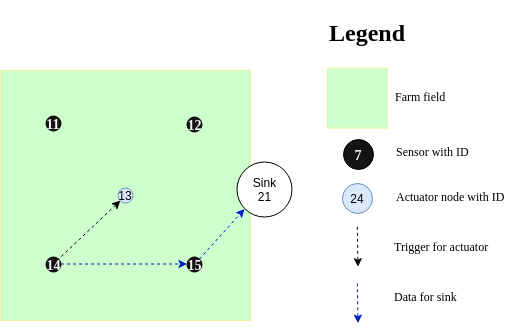
\includegraphics[width=0.5\linewidth]{images/actuate}
	\caption{Communication patterns in agricultural WSN}
	\label{fig:actuate}
\end{figure}

A reactive protocol was chosen for communication between zones in order to limit the amount of network knowledge required for routing. It also has the benefit that link breakages do not need to be broadcast to the entire network, and can instead only be sent to nodes relying on that links existence at the time of breakage.

A proactive protocol was chosen for routing within locators as it would provide node discovery, and would hopefully reduce the number of repeated route discoveries after breakages by being able to find alternative routes within zones.

\subsection{Intra-Zone Routing Protocol}

Initially, each node broadcasts its presence to its neighbours in order to learn what links were available to it using a \emph{Hello} message, containing its lambda value. 

Neighbouring nodes reply with their current link state database (LSB) in a \emph{LSBMessage}. This message contains the neighbouring nodes knowledge of the internal (within the locator) topology, as well as the links to external networks (other locators). Figure \ref{fig:lsbexchange} gives a simple example of this communication. Whilst still in the intiliziation phases, neighbours will flood their entire LSBs to their neighbours, and once the messages they receive contain match their own LSBs, they can be considered initialized. This ensures that every node in the network has the same database and is aware of all other nodes in the network.

\begin{figure}[!ht]
	\centering
	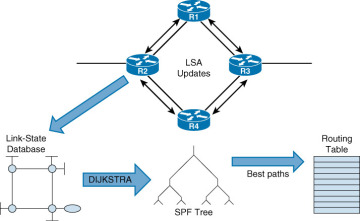
\includegraphics[width=\linewidth]{images/ldb}
	\caption{Exchange of LSB messages when a new node joins.}
	\label{fig:lsbexchange}
\end{figure}

Nodes that exist on the border of locators will discard LSBs they receive from the locators they are not part of. They will however use these messages to learn what other locators can be reached from their neighbours, eventually providing them with next hops for all locators in the WSN.

Once converged and the entire local topology is available, data packets would be routed using the following logic:

\begin{enumerate}
	\item If the packet destination ID matches the current node, then it will add the payload of the packet to the received queue. 
	\item Otherwise it will attempt to find the next hop for the packet, provided by the forwarding table, and forward it to the node with that ID. 
	\item If no entries are found in the forwarding table:
	\begin{enumerate}
		\item If the packet destination locator matches this nodes locator, then not finding a next hop suggests that the destination ID doesn't exist, and so the packet is discarded. 
		\item Otherwise, the inter-zone routing protocol will be invoked, but only if the packet originates from the current node. 
	\end{enumerate}
\end{enumerate}

This method ensures that packets arriving from external locators will receive best effort routing based on the assumptions that:

\begin{enumerate}
	\item All nodes within a locator have at least one path between each other. 
	\item Data packets are only sent to other locators once a route has been established.
\end{enumerate}

Whenever a link is detected as being lost due to the lack of keepalive messages after a period of time, then this information will be shared within the network. A \emph{ExpiredLink} message will be broadcast, and flooded by nodes within the same locator in order to remove the link from their network, or to inform the other nodes that a neighbouring locator is no longer accessible via a given link.

\subsection{Inter-Zone Routing Protocol}

AODV is a reactive protocol that is used differently for inter-zone and inter-zone routing. Inside locators, the hop list will consist of node IDs, providing exact routes between the source and destination. Between locators, the hop list will consist of locators, and the exact hop-by-hop routing will be provided by each zone internally.

AODV has three phases: discovery, maintenance, and recovery.

To discover routes to a given destination, AODV produces a list of hops that a packet can be sent over to reach a destination by flooding route request packets (RREQs). The route discovery process is summarised in figure \ref{fig:path}, where the leftmost node (1) is requesting a route to the rightmost node (4).

\begin{figure}[!ht]
	\centering
	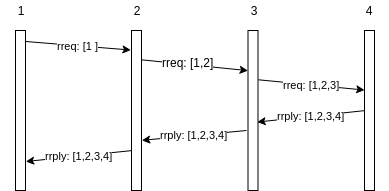
\includegraphics[width=\linewidth]{images/path}
	\caption{Route Discovery Overview}
	\label{fig:path}
\end{figure}

Figure \ref{fig:rreqflow} shows how RREQs are processed at each node. The destination node replies to all route requests for it, as this can provide multiple paths to the requesting node. Intermediate nodes however only forward requests based on whether or not they've seen them already. This can be established based on the request ID, which coupled with the source ID in the ILNP packet header can identify duplicate requests. Otherwise if this node's identifier already appears in the path so far, then it can also be discarded. These checks reduce unecessary duplication of request packets and avoid loops in the resulting paths.

When using ILNP instead of IP with AODV, packets can be routed based on the identifier alone, and this can result in multiple paths to the same node. This provides robust communication if the end destination is multihomed (i.e. has interfaces to multiple locators), with less complexity than in IP. It also makes it easier to identify disjoint paths as the node has a single name in the network, which wouldn't be the case in IP multihoming. 

\begin{figure}[!ht]
	\centering
	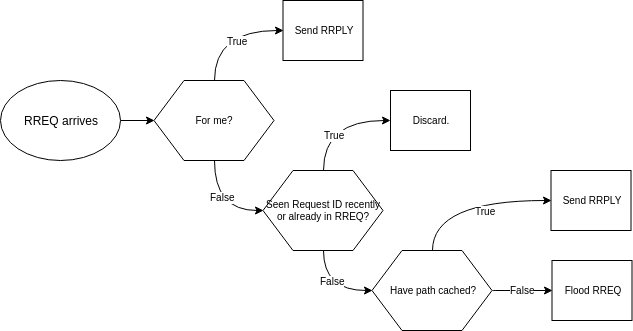
\includegraphics[width=\linewidth]{images/rreqflow}
	\caption{Route Request (RREQ) Flow}
	\label{fig:rreqflow}
\end{figure}

Once the RREQ reaches its destination, or any intermidiate node that already has a path cached to the that destination, a Route Reply (RRPLY) is generated by copying the full path from the RREQ or route cache and sending it back along the same path it arrived to the requesting node. Figure \ref{fig:rrplyflow} shows the processing that occurs at each node.

By forwarding RRPLYs along the reverse of the path that they contain, we ensure that the route hasn't broken between creation and reception of the route request. Intermediate nodes can filter erraneous route replies by only considering those where they know the next hop neighbour is still available.

This only works if we assume that all links are bidrectional which is not always the case especially in heterogenous WSNs, due to differences in transceiver ranges. 
\cite{unidirec} shows that accounting for unidirectional links in a protocol does not provide much benefit compared to the increased overhead. Also in our scenario, the nodes are likely to be homogenous and evenly spaced, so transceiver power can be assumed to be equal throughout, with no interference hot spots. 

\begin{figure}[h]
	\centering
	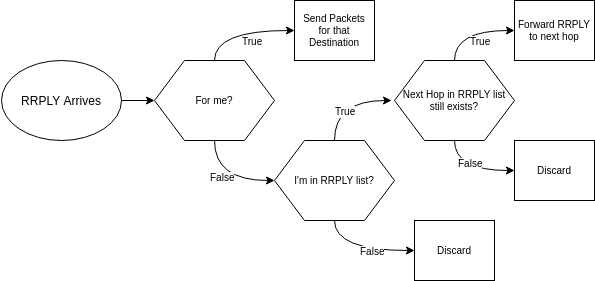
\includegraphics[width=\linewidth]{images/rrplyflow}
	\caption{Route Reply (RRPLY) Flow}
	\label{fig:rrplyflow}
\end{figure}

The structure of the route request is the same as in RFC3561 \cite{aodv}, but with an extra $\lambda$ field in the header. This value provides a metric for determining the lifespan of a route, and is calculated for an individual node using equation \ref{eq:lambda}, and visualised in Figure \ref{fig:lambda}. 

\begin{equation} \label{eq:lambda}
	\lambda = 1 -(1 - E)^2
\end{equation}

where $L$ is the \% of load the node is willing to give to networking, and $E$ is the \% battery remaining. It is based on the equation for $\lambda$ in \cite{groups}, adjusted so that $E = 0$ occurs when the battery is empty. 
The effect of decreasing $E$ was chosen so that the value of $\lambda$ would be similiar during network initialization, but to avoid network partions smaller values of $E$ would have a greater effect on $\lambda$.
Each node calculates this value before adding their ID to the path in the RREQ, and only changes the field in the packet if its calculated value is lower. 

\cite{groups} also included a load balancing factor that would account for the number of neighbours a node had, and this was considered for use in the AODV implementation. Instead of using the number of neighbours as in their link state protocol, we could use the number of nodes using a route that passed through this node. 
This value could be ascertained by counting the number of unique source IDs of packets that were forwardded. However, defining a maximum in order to normalise this factor would place restrictions on how large the network could grow. Too large and the factor has no real effect, too small and it would reduce to zero making the metric meaningless for nodes further upstream. If this number could be supplied however, it would help other nodes choose routes that aren't being used as heavily, which would be very beneficial for the lifespan of the network.

\begin{figure}[h]
	\centering
	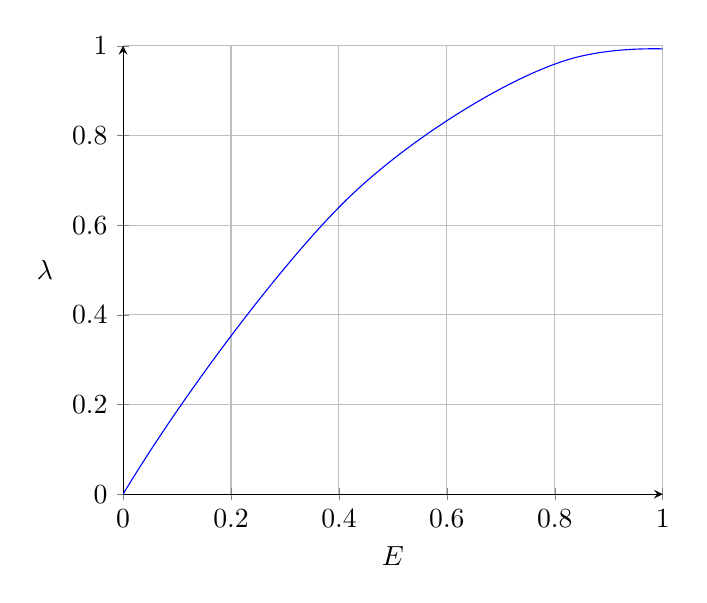
\begin{tikzpicture}
%		\begin{axis}[set layers,view={90}{0},
%			 axis lines=left,
%			 grid=major,
%			 no marks,
%			 xmin=0, xmax=1, xlabel=$E$,
%			 ymin=0, ymax=1, ylabel=$\lambda$, ylabel style={rotate=-90}
%			 ]
%			\addplot+[smooth,blue] {1 - (1 - x)^2}; % actual curve
%			\begin{pgfonlayer}{pre main}
%				\clip plot[variable=\x,samples=25,domain=0:1] (\x,{1 - (1 - \x)^2})
%				|-cycle;
%				\node at (0.5,0.5){\usebox\backbox};
%			\end{pgfonlayer}
%			% filling
%		\end{axis}
		\begin{axis}[set layers,view={90}{0},
			 axis lines=left,
			 grid=major,
			 no marks,
			 xmin=0, xmax=1, xlabel=$E$,
			 ymin=0, ymax=1, ylabel=$\lambda$, ylabel style={rotate=-90}
			 ]
			\addplot+[smooth,blue] {1 - (1 - x)^2}; % actual curve
		\end{axis}
	   \end{tikzpicture}
	   \caption{Plot of Equation \ref{eq:lambda}}
	\label{fig:lambda}
\end{figure}

In order to check if neighbours are still live, \emph{HELLO} messages are exchanged at regular intervals between neighbouring nodes. These messages also provide neighbour discovery as they are limited to one hop, therefore the source ID can be mapped to the arriving IPv6 address in the emulated link layer. 

\begin{figure}[!ht]
	\centering
	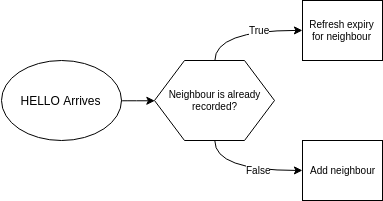
\includegraphics[width=0.6\linewidth]{images/helloflow}
	\caption{Hello Flow}
	\label{fig:helloflow}
\end{figure}

Figure \ref{fig:helloflow} shows how the \emph{HELLO} messages are processed. If a node fails to deliver a hello messages after a certain interval, then it's neighbours will begin the route recovery process.

Cached routes will also expire after some time to trigger another route request if required. This allows nodes to learn if a path is under heavy load, and ensures that a route will be corrected if for some reason the recovery process is not completed. 

If the keepalive process fails for a neighbour, then a node will forward a RERR to all previous nodes in any paths it takes part in, shown in figure \ref{fig:rerrflow}.

\begin{figure}[h]
	\centering
	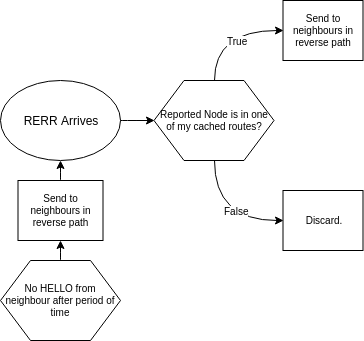
\includegraphics[width=\linewidth]{images/rerrflow}
	\caption{Route Error (RERR) Flow}
	\label{fig:rerrflow}
\end{figure}

Any packets that were sent between the failure of the link and the receiving of a route error will most likely be dropped, and future packets will be delayed as route discovery will have to take place again unless this node is aware of a disjoint path to the destination.

% TODO Merge this into sections talking about that part of the protocol

The intra-zone routing table is responsible for forwarding packets between the nodes of a locator. To do this, it keeps track of:

\begin{enumerate}
	\item The destination node ID
	\item The next hop ID to reach the destination ID
	\item The cost of this path, based on $\lambda$.
	\item Whether or not the destination node is a border or normal node.
	\item The neighbouring locators that the destination node has links to (border nodes only).
\end{enumerate}

The intra-zone routing table is built by broadcasting RREQs where each hop is an node ID, and only contains routes to actuator nodes and border nodes. 

% TODO Merge this into sections talking about that part of the protocol

The inter-zone routing table is responsible for forwarding packets between nodes in different locators, and is maintained by nodes that exist on the borders of these locators such as those highlighted red in figure \ref{fig:border}. It contains information about:

\begin{enumerate}
	\item The destination locator 
	\item The next hop locator to reach this destination (i.e the ID of a border node from a neighbouring locator)
\end{enumerate}

If multiple border nodes provide links to the same neighbour zone, then nodes will alterate between them using a weighted round robin method based on the path costs to avoid all traffic travelling through the same border node.

When packets arrive to be forwarded to another locator, the interzone forwarding table will be used to find the next hop locator. Then the intrazone forwarding table will be used to provide the next hop ID in order to reach a border node that can get the packet closer to the destination locator;

\begin{figure}[!ht]
	\centering
	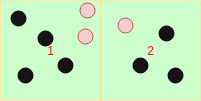
\includegraphics[width=0.5\linewidth]{images/nb}
	\caption{Border Nodes}
	\label{fig:border}
\end{figure}

Figure \ref{fig:external} shows locator discovery occuring, which returns the locator of the destination node with the requested ID, and the hop by hop list of locators that have to be crossed to reach it.
Once this locator discovery has been carried out, border nodes will be aware of how to reach each locator, and so will be able to forward packets to that destination.

\begin{figure}[!ht]
	\centering
	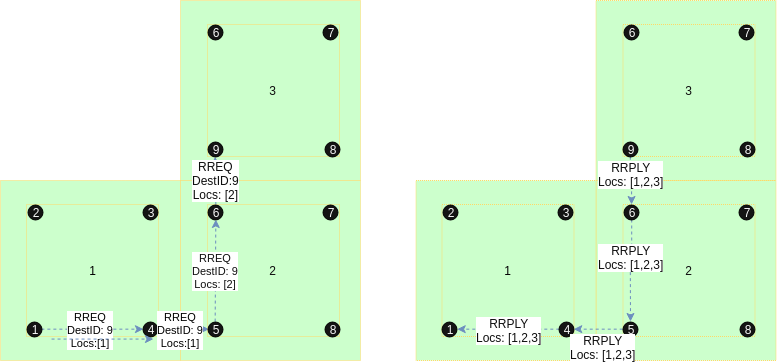
\includegraphics[width=0.8\linewidth]{images/external}
	\caption{Locator Discovery}
	\label{fig:external}
\end{figure}

\FloatBarrier
\pagebreak
\section{ILNP Testbed Implementation}

Due to the recency of ILNPv6, there does not currently exist software for emulating wireless ILNP networks as there is for IP, therefore a custom testbed had to be implemented.  

The testing environment was implemented using Python 3.7. The project has three main components: The wireless network emulation, routing and network management, and sensor emulation. Figure \ref{fig:struc} shows the components with the flow of messages.

\begin{figure}[!ht]
	\centering
	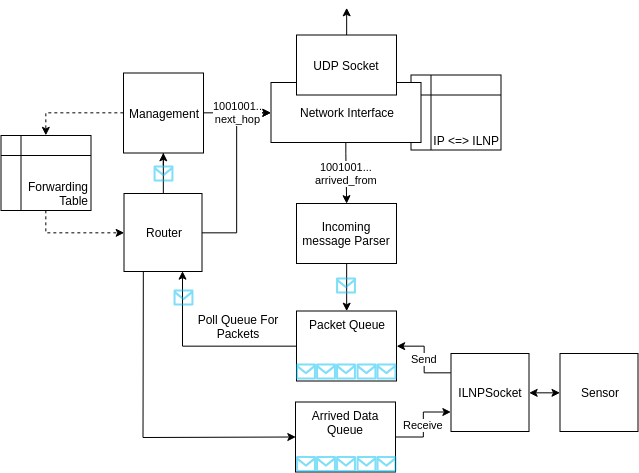
\includegraphics[width=\linewidth]{images/struc}
	\caption{Implementation Structure}
	\label{fig:struc}
\end{figure}

Emulating wireless communication was achieved by building an overlay network using UDP with multicast. A single UDP socket provided a communication endpoint.

A multicast group exists for each node ID, and so neighbours of a node would join the multicast groups of their neighbours in order to receive broadcasted packets. Figure \ref{fig:mcast} shows the ranges of each sensors radio signal as dashed lines, where each node within the range joins the multicast group.

\begin{figure}[!ht]
	\centering
	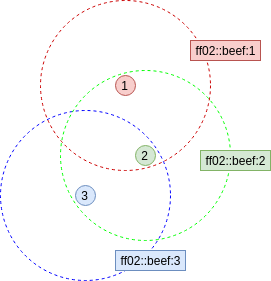
\includegraphics[width=0.5\linewidth]{images/mcast}
	\caption{Wireless broadcast emulation using multicast}
	\label{fig:mcast}
\end{figure}

IPv4 uses the Address Resolution Protocol (ARP) and IPv6 uses Neighbour Discovery (ND) in order to produce a mapping between IP addresses and the link layer addresses of other machines in a local network. In our overlay network, the IP addresses of the underlying network could be treated as MAC addresses. This would allow us to emulate neighbour discovery in ILNPv6, and provide unicast communication once a mapping between these virtual link layer addresses and ILNP IDs were obtained via broadcasted messages. 

The network interface abstraction provided the following methods:
\begin{enumerate}
	\item \textbf{send}: For unicast communication.
	\item \textbf{broadcast}: For establishing neighbours or flooding packets.
	\item \textbf{receive}: For receiving packets, broadcast or unicast.
\end{enumerate}

A daemon thread continuously polls the network interface for incoming data. It then parses the contents of the packet and records the source IDs and source IP addresses of any neighbourhood discovery packets for later communication. 

All polling functions included a timeout in order for each thread to check if it has been asked to terminate, if for example the power levels had reached a critical level.

The router polls the incoming packet queue and decides the next course of action. 

The control plane handles any control packets or any packets that can't be forwarded using the current forwarding table, and is responsible for populating the forwarding table.

\#https://ieeexplore.ieee.org/document/7993954 to fix route reply storm issue: add jitter before responding with route reply and listen for other replies

The sensor initialises the ILNPSocket, and depending on whether or not it is configured to operate as the sink (where all the data from every node is collected) begins either polling for packets or sending 'readings' at intervals.

To mock realistic application data, a random fluctuation is applied to a series of values that would be relevant in our scenario: temperature, humidity, pressure, and luminosity \cite{agrisensor}.

Only the ID of the sink is known by each node, which is all that should be necessary when using ILNP to route a packet. If it was possible to provide a FQDN for the sink node then the addressing scheme would be abstracted also, but emulating a DNS was deemed unecessary for the experiment.

\pagebreak
\section{Experiment}

The aims of the experiment were to show that protocol succeeded in meeting the goals from section \ref{ssec:goal}, and to exemplify how ILNP helped in achieving these goals compared to how it would be implemented in IP. This was be achieved by simulating a wireless sensor network for monitoring fields in a farm. 

Figure \ref{fig:layout} shows the real life scenario being emulated, where each black circle represents a sensor node, and the green circles represent interfaces to the sink, such as be wireless receivers. The transparent red circles represent the wireless ranges of the nodes, and the blue dotted arrows show  an example path that could be taken to reach the sink.

For the emulation, we assumed that: 
\begin{enumerate}
    \item Each sensor had equal radio ranges.
    \item Sensors always listened for packets with same antennae (i.e. no lower power antennaes would be used until a signal was detected\cite{offon})
    \item Sending a packet has a fixed energy cost, regardless of size of payload.
    \item Collisions and interference would not occur.
\end{enumerate}

\begin{figure}[!ht]
	\centering
	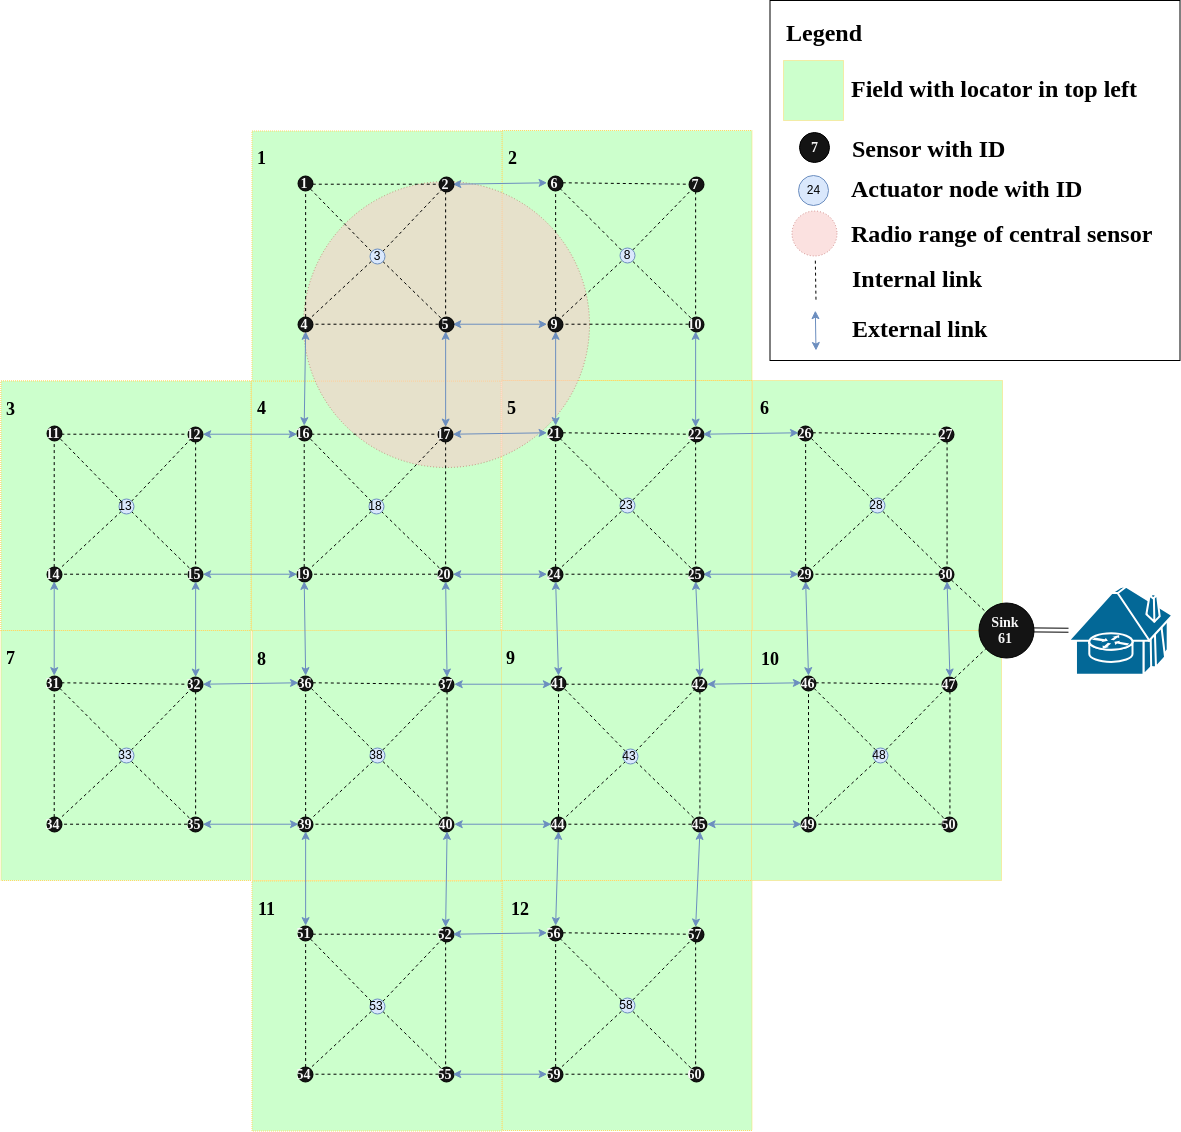
\includegraphics[width=\linewidth]{images/layout}
	\caption{WSN layout with example routes.}
	\label{fig:layout}
\end{figure}

Two experiments would be run in order to compare performance when using ILNP and IP. The hypothesis being that the protocol will perform better using ILNP since nodes will be able to operate without knowledge of the entire network. Figure \ref{fig:spectrum} shows that ILNP can emulate IP by either:
\begin{enumerate}
	\item providing a locator for every node, essentially treating every node as a subnetwork that will require a routing table entry.
	\item using the same locator for all nodes, which would require knowledge of the entire subnetwork in order to route correctly.
\end{enumerate}

Both extremes of the spectrum will provide identical flat addressing schemes like IP, so either could be used to the same effect. The locator per node approach was taken for this experiment.

\begin{figure}[!ht]
	\centering
	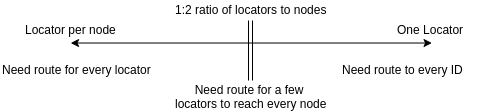
\includegraphics[width=\linewidth]{images/spectrum}
	\caption{Relationship between IP and ILNP}
	\label{fig:spectrum}
\end{figure}

\subsection{Setup}

The experiment was run on the lab machines, remaining within the schools network. 

To construct and automate the testing environment, a series of bash scripts were written. The first of which would perform a quick liveness check using a list of IP addresses of the lab machines in order to know which machines were available for use.

Since multicast was being used to emulate wireless broadcast, my user ID was used as the second-last octet to avoid collision with other experiments possibly running on the network.

The configuration files that were used to initialize each sensor node were generated by performing string replacement on a template configuration. "LOC\_1\_ID\_2\_MCAST\_1\_2" for example would produce a configuration file for a node with ID 2, locator 1, that was part of the multicast groups "ff02::dead:1" and "ff02::dead:2". Being able to describe network topologies using single strings allowed multiple tests to be configured easily, and possible future work could involve generating these configurations using a visual representation of the network.

With the list of available computers and the configuration files generated, another script was written that would \emph{ssh} into the lab machines one by one and start the sensor emulation program with each configuration. Logs from each instance of the program were redirected to a file based on the node ID for monitoring the network.

\subsection{Method}

In order to monitor the type and number of packets sent and forwarded by each node, an additional \emph{monitor} module was added to the testbed implementation. For each packet sent, the monitor recorded a the ID of the sensor, timestamp, the type of packet (control or data), and whether or not the packet originated from this node or was being forwarded. The monitor would also report the size of the routing table when each packet was sent. 

Using this information, the flow of packets over time could be visualised, and the ratio of control packets to data packets (i.e. overhead) could be measured. 

The sink node would also record each data packet it received, which included a sequence number so that the level of disordering and packet loss that occurred could also be measured. Loss would simply be the difference between the number of data packets sent by each sensor and the number received by the sink. Disorder was measured as the absolute different between the current highest sequence number received from a node (i.e the sequence number in the most recently sent packet) and the sequence number in the received packet.

A \emph{battery} module was also added to the emulation. The battery would be decremented as each packet was sent, emulating real loss of power when transmitting which would be used when calculating $\lambda$ for each node.

Each test was run multiple times in order to ensure that the results were consistent.

\subsection{Results}

Figures \ref{fig:datasnapone} and \ref{fig:ctrlsnapone} show the concentration of data and control packets throughout the network during the intialisation of the network in the multiple sink scenario. As expected, the overhead is initially quite high, as every node is trying to learn routes to the sink. 

\begin{figure}[!ht]
    \centering
    \begin{minipage}{0.45\textwidth}
        \centering
        \includegraphics[width=0.9\textwidth]{example-image-a} % first figure itself
        \caption{Data packets sent by each node during network initialisation.}
        \label{fig:datasnapone}
    \end{minipage}\hfill
    \begin{minipage}{0.45\textwidth}
        \centering
        \includegraphics[width=0.9\textwidth]{example-image-b} % second figure itself
        \caption{Control packets sent by each node during network initialisation.}
        \label{fig:ctrlsnapone}
    \end{minipage}
\end{figure}

Figures \ref{fig:datasnaptwo} and \ref{fig:ctrlsnaptwo} show how the overhead decreases once routes are established, and how the paths taken are fairly evenly spread and not just focused around the shortest paths. 

\begin{figure}[!ht]
    \centering
    \begin{minipage}{0.45\textwidth}
        \centering
        \includegraphics[width=0.9\textwidth]{example-image-a} % first figure itself
        \caption{Data packets sent by each node once initial routes have been established.}
        \label{fig:datasnaptwo}
    \end{minipage}\hfill
    \begin{minipage}{0.45\textwidth}
        \centering
       \includegraphics[width=0.9\textwidth]{example-image-b} % second figure itself
        \caption{Control packets sent by each node once intial routes have been established.}
        \label{fig:ctrlsnaptwo}
    \end{minipage}
\end{figure}

Figures \ref{fig:datasnapfour} and \ref{fig:ctrlsnapfour} show how as nodes begin to fail, the limited number of paths force heavier traffic to pass through the remaining nodes. The failing nodes have occurred near the sinks as expected.

\begin{figure}[!ht]
    \centering
    \begin{minipage}{0.45\textwidth}
        \centering
        \includegraphics[width=0.9\textwidth]{example-image-a} % first figure itself
        \caption{Data packets sent by each node once failures have started to occur.}
        \label{fig:datasnapfour}
    \end{minipage}\hfill
    \begin{minipage}{0.45\textwidth}
        \centering
        \includegraphics[width=0.9\textwidth]{example-image-b} % second figure itself
        \caption{Control packets sent by each node once failures have started to occur.}
        \label{fig:ctrlsnapfour}
    \end{minipage}
\end{figure}

Figure \ref{fig:loss} shows the packet over time, and finally figure \ref{fig:dis} shows the level of disordering over time.

\begin{figure}[!ht]
    \centering
    \begin{minipage}{0.45\textwidth}
        \centering
        \includegraphics[width=0.9\textwidth]{example-image-a} % second figure itself
        \caption{Packet loss over time.}
        \label{fig:loss}
    \end{minipage}\hfill
    \begin{minipage}{0.45\textwidth}
        \centering
        \includegraphics[width=0.9\textwidth]{example-image-b} % second figure itself
        \caption{Disordering over time.}
        \label{fig:dis}
    \end{minipage}\hfill
\end{figure}

\FloatBarrier
Figure \ref{fig:internaltablesize} shows the sizes of the internal forwarding tables for IP and ILNP, and \ref{fig:externaltablesize} shows the sizes of the external forwarding tables.

\begin{figure}[!ht]
    \centering
    \begin{minipage}{0.45\textwidth}
        \centering
        \includegraphics[width=0.9\textwidth]{example-image-a} % second figure itself
        \caption{Sizes of internal forwarding tables over time.}
        \label{fig:internaltablesize}
    \end{minipage}\hfill
    \begin{minipage}{0.45\textwidth}
        \centering
        \includegraphics[width=0.9\textwidth]{example-image-b} % second figure itself
        \caption{Sizes of external forwarding tables over time.}
        \label{fig:externaltablesize}
    \end{minipage}\hfill
\end{figure}

\FloatBarrier

\section{Discussion}

\begin{enumerate}
\item Explain features of heat map and snapshots
\item Discuss how well the routing protocol performed, compared to other implementations. 
\item Discuss weaknesses with experiment
\end{enumerate}

\pagebreak
\section{Conclusions}

Discuss how global AODV was originally considered, but discarded since it didn't take full advantage of ILNP.

Possible mercy message to send from nodes under heavy load to try and request downstream nodes to use different paths, rather than outright route errors.

was the goal met, and if so how well?

future work with ILNP, possible suggestions of better alternatives to the routing protocol used.

\pagebreak
\section{Appendix}
\begin{enumerate}
\item Instructions on installing, and executing and using the python module
\end{enumerate}

\bibliographystyle{unsrt}
\bibliography{mybib}

\end{document}
